\chapter{Background} \label{background}
Polyps are small growths found in and around the inner lining of the large intestine. These polyps, also referred to as adenomas, can in time develop into cancerous tumors, or carcinomas, in a process known as the adenoma-carcinoma sequence~\cite{ACS}. Though the majority of polyps do not undergo this process, identifying polyps nonetheless constitutes an important step towards preventing colorectal cancer. Indeed, resection of these polyps has been shown to reduce the incidence of colorectal cancer by a significant margin~\cite{resection}. 

Though colorectal cancer remains as one of the leading causes of cancer-related death worldwide~\cite{colorectal_cancer}, mortality rates have in recent years declined in large part to the increased use of screening colonoscopy and subsequent preemptive treatment~\cite{screening}. Polyps are by nature somewhat difficult to detect, however, and are routinely missed by clinicians, with miss rates reportedly ranging upwards of $27\%$ for diminutive (<2.5mm) polyps~\cite{missrate1, missrate2}.
\begin{figure}
    \centering
    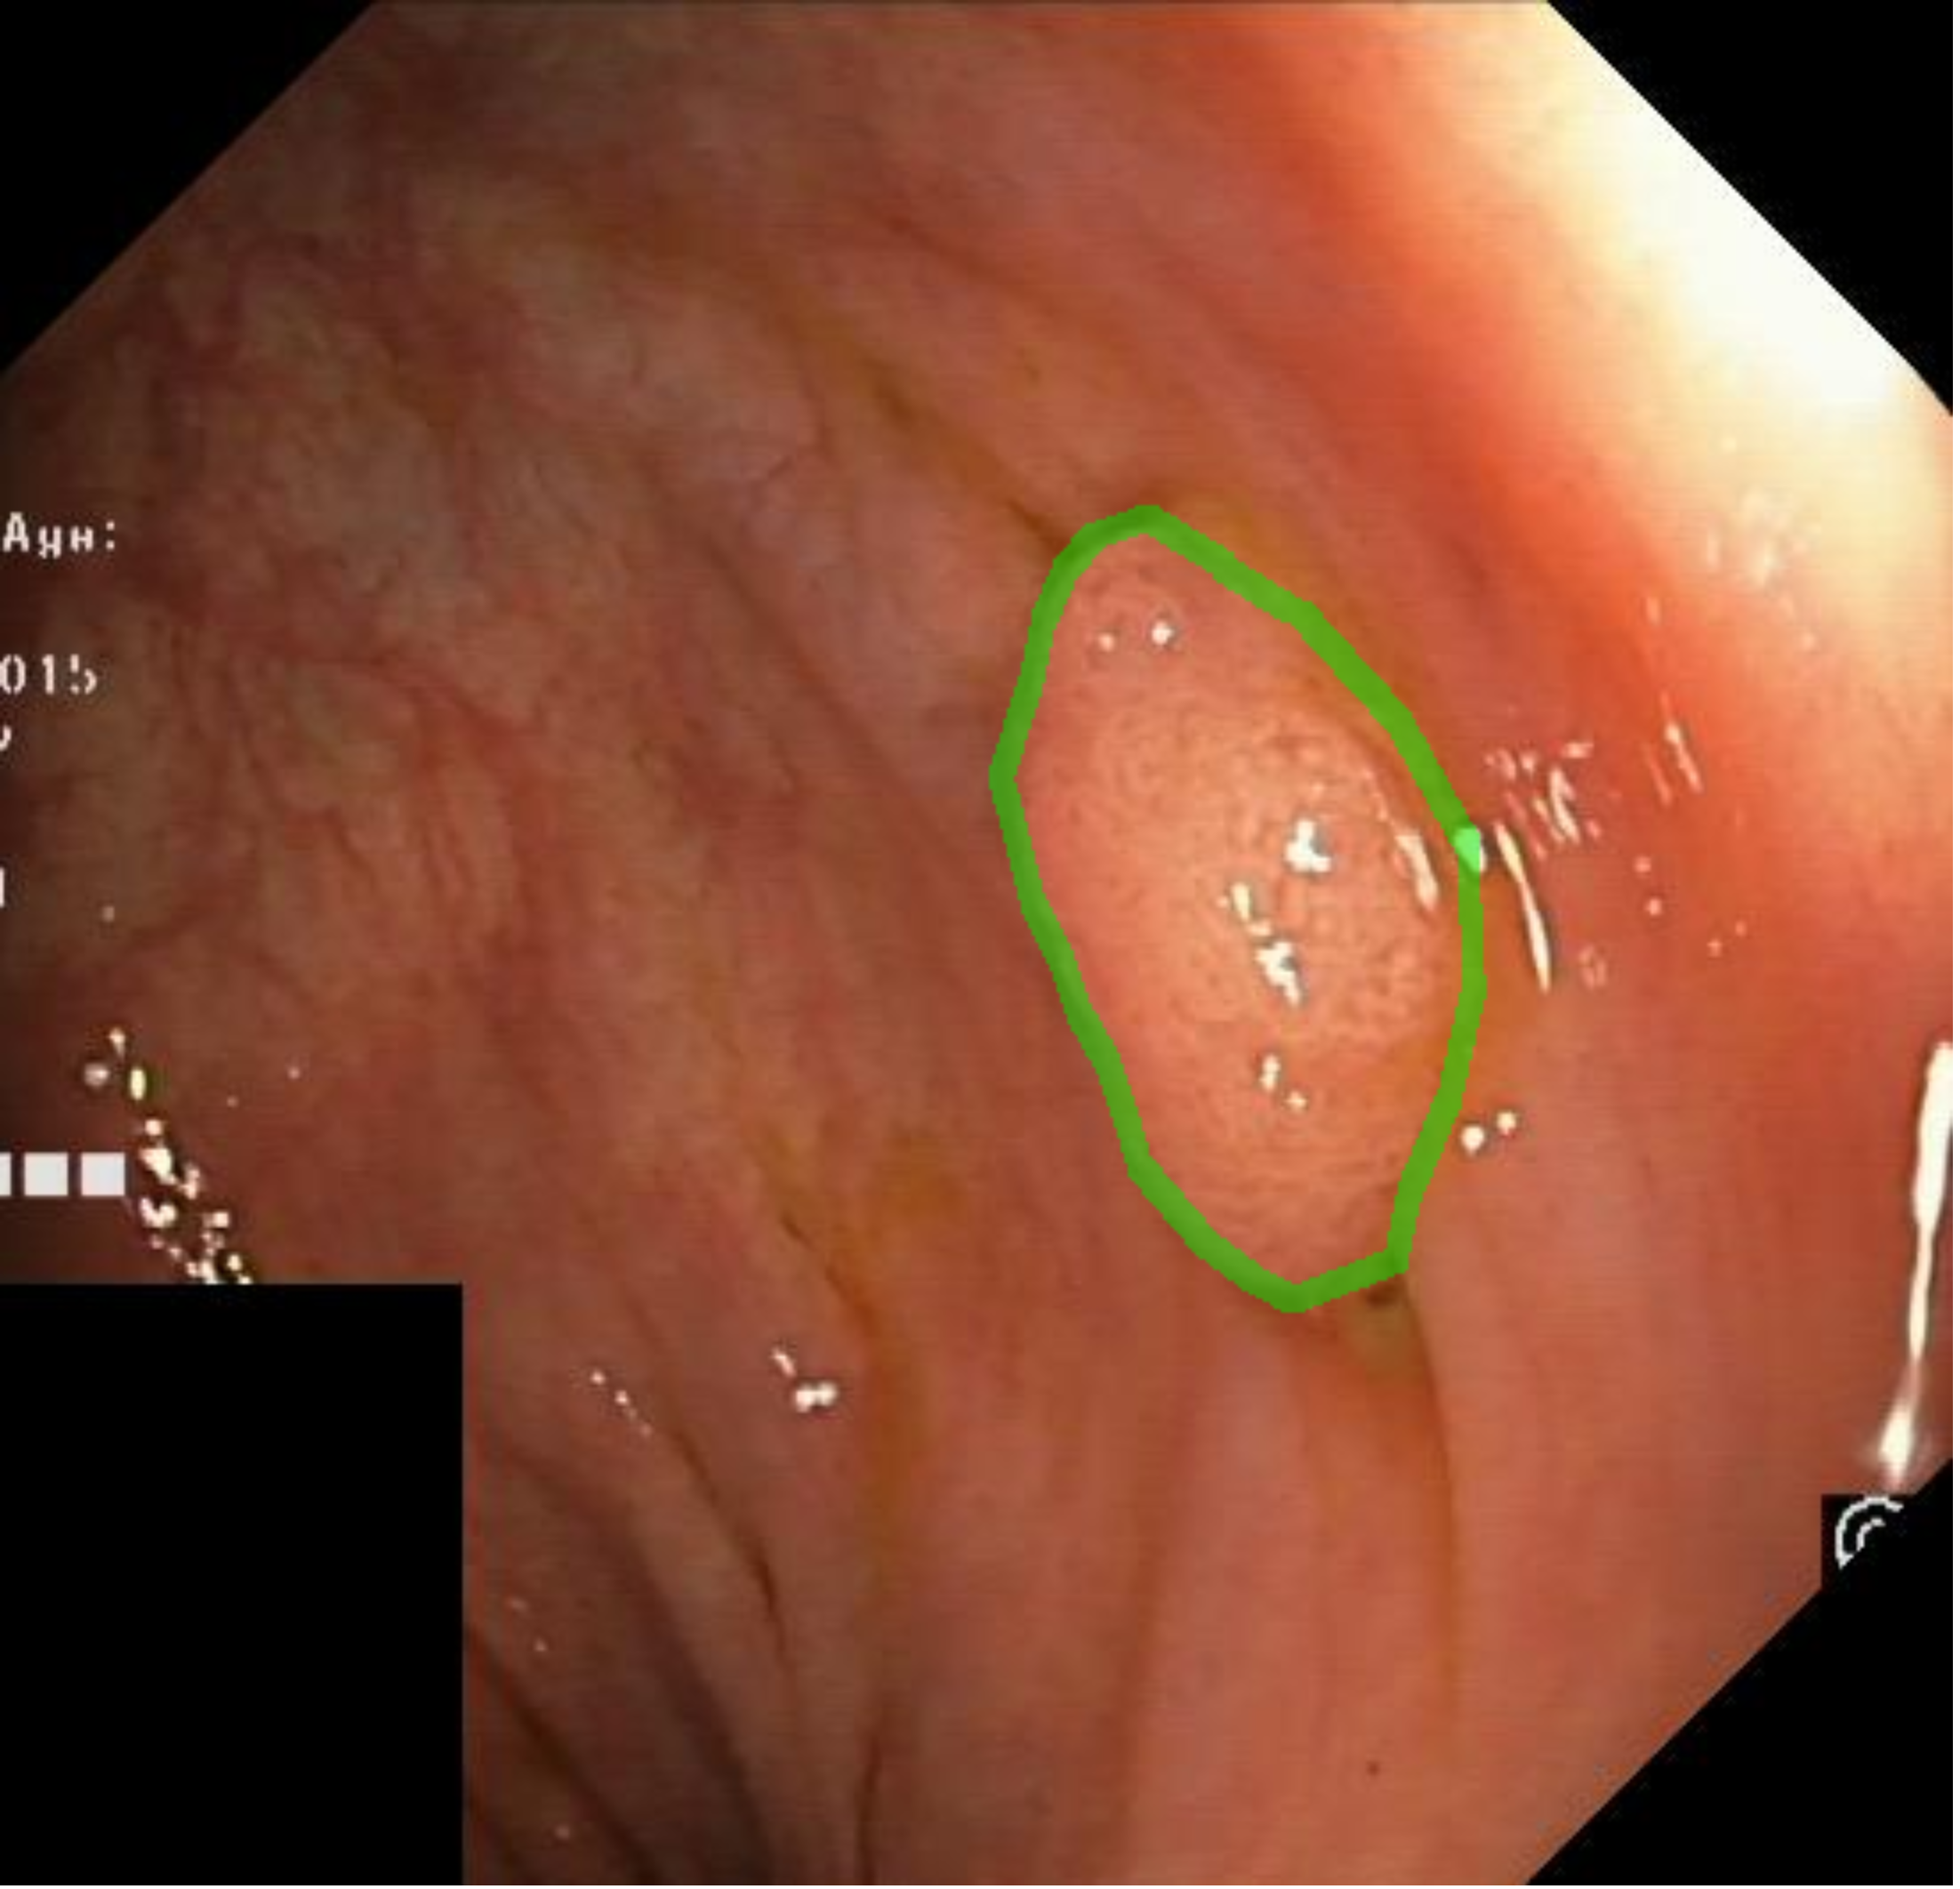
\includegraphics[width=0.75\linewidth]{illustrations/polyp.png}
    \caption{Example of a colorectal polyp from the Kvasir-SEG~\cite{kvasir} dataset. The polyp is outlined in green.}
    \label{fig:polyp}
\end{figure}
Reducing this miss rate has the potential to further reduce the incidence of colorectal cancer. As a result, there has been a significant body of work dedicated to developing systems and techniques to aid in more accurate screening. Certain image-processing techniques, namely I-SCAN, have for instance been shown to reduce miss-rates by up to $50\%$~\cite{i-scan}. Similarly, the use of narrow-band imaging, wherein light of specific wavelengths specifically designed to highlight the textural differences between the polyps and the surrounding tissue, have been shown to reduce miss rates by 26\%~\cite{nbi}. 

These systems do, however, require specialized equipment, training and expertise to effectively employ. Thus, automatic polyp detection using \glspl{dnn}, and in particular \glspl{cnn}, has also been identified as a possible ancilliary screening method. This requires minimal training time on the part of the clinician, no additional equipment, and has been shown to increase detection rates by 10\% when deployed in a clinical setting~\cite{polyp-success-story}. 

This has spurred on a large body of research dedicated to improving the performance and expanding the capabilities of deep-learning based systems for polyp detection and segmentation. Several challenges been also held, namely the Endotect Challenge~\cite{endotect}, EndoCV2020~\cite{endocv2020} and EndoCV2021~\cite{endocv2021}.

There are, however, still several hurdles to overcome; recent research has shown that even state of the art deep-learning pipelines are prone to generalization failure when deployed in practical settings, particularly when exposed to distributional shifts such as changes in demographics, imaging equipment, noise, and more despite exhibiting high performance on hold-out sets~\cite{retinopathy, damour2020underspecification, pneumonia, shortcut_learning}. This was further highlighted in the EndoCV2021 challenge, wherein submissions were evaluated on a hidden dataset collected from a different hospital than the training data. Though many of the submissions exhibited increased generalizability when compared to baseline models, significant performance gaps were nonetheless present, highlighting that generalization failure remains an open and highly challenging problem~\cite{endocv2021}. 

Understanding how and why such generalization failure occurs and developing methods to counteract it is a subject of ongoing study. This chapter will attempt to summarize and synthesize recent findings in the field. It will first cover the necessary understanding of deep learning and segmentation, before moving on to a survey over instances of generalization failure both in systems dedicated to polyp-segmentation and other applications of deep learning. These failures will then be analyzed through the lens of generalizability theory, starting from the theoretical fundamentals underpinning deep learning - namely \glsfirst{erm} - and incorporating recent analyses in the literature pertaining to generalizability failure and its origins. Finally, recent work on generalizable methods will be summarized, and analyzed with respect to the aforementioned theory. 
	
\section{Deep Learning}
The past decade or so has seen considerable advancements in Deep Learning. This has facilitated significant performance improvements for various tasks across a wide range of domains - ranging from computer vision~\cite{computer_vision} - polyp segmentation included - to finance~\cite{dl_finance}, and from natural language processing used for tasks like machine translation~\cite{dl_nlp}, to the content recommendation engines used by most social media platforms~\cite{dl_recommend} and even to complex tasks like robot-control~\cite{dl_robotics} and games like Chess and Go~\cite{dl_go}. 

To fully explain how and why Deep Learning performs so well - and why it sometimes does not - this section will cover the basics of Deep Learning and the Deep Learning Pipeline. It will also detail the problem of semantic segmentation in the context of polyps, and finally describe how a Deep Learning Pipeline can be adapted to try to solve this problem.

\subsection{The Deep Learning Pipeline}
    Deep Learning is a supervised machine learning method, wherein a \glsfirst{dnn} - typically consisting of millions and even hundreds of billions of parameters - learns to identify patterns conducive to approximating the mapping between pairs of inputs and labels given by a dataset~\cite{deep_learning_book}. Conceptually, one can consider \glspl{dnn} as general-purpose correlation machines; i.e that they accept some paired input-output data, learn correlations between the inputs and outputs and then predict according to these correlations at inference-time. Similar to how one can us establish linear relationships by performing linear regression on a set of (linearly) related variables, \glspl{dnn} are capable of establishing non-linear relationships via Deep Learning given paired input-output data. The inputs can for instance be images and the outputs categories - also referred to as classes -, bounding boxes, or -as in the case of segmentation - regions, or the inputs could be sentences in English and the outputs sentences in French. So long as the data can be encoded into a vector-space, deep learning can typically be applied. 
    
    This is achieved through a process known as training, the objective of which is to adjust the parameters of the \gls{dnn} such that the model exhibits maximal performance. Training a \gls{dnn} is naturally not straight-forward; each parameter corresponds to a dimension in the search space, and searching through millions upon millions or more dimensions in order to find a sufficiently performant parameter configuration is a challenging problem. Deep Learning systems nevertheless achieve this through a process known as gradient descent~\cite{gradient_descent_overview}. Fundamentally, this involves minimizing some quantity inversely proportional to whatever performance metric one seeks to maximize. This quantity is referred to as the \textit{loss}, and the function that generates it a \textit{loss function}. Minimizing the loss is achieved by differentiating the loss function with respect to the model's parameters and adjusting them in the direction of the gradient. There are, naturally, a number of complicating factors involved in this process, which through nearly a decade of research have been addressed using a number of different techniques culminating in what will be referred to as the \textit{deep learning pipeline}. The constituent components thereof, as well as further technical details as to how \glspl{dnn} are trained, will be further described in the following paragraphs, and are illustrated in~\Cref{fig:pipeline}. 
    
    \begin{figure}[h]
        \centering
        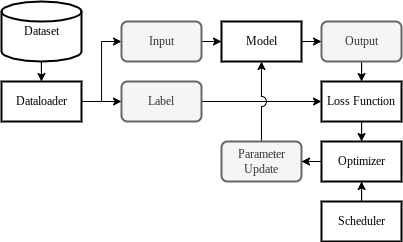
\includegraphics[width=0.75\linewidth]{illustrations/pipeline.png}
        \caption{Conventional Deep Learning pipeline}
        \label{fig:pipeline}
    \end{figure}
    
    \subsection{Architectures and Models}
        The \gls{dnn}, typically referred to simply as the \textit{model}, can be considered the central component of the deep learning pipeline. There are several types of \glspl{dnn}, including \glspl{rnn}~\cite{rnns}, Transformers~\cite{transformer}, \glspl{mlp}~\cite{neural_nets}, and \glspl{cnn}~\cite{cnn_survey}. Common to all of the aforementioned types is that they consist of multiple instances of similar functional blocks, often called layers, which are connected to one another. A \gls{mlp} consists of layers of perceptrons, a \gls{rnn} primarily consists of stacked recurrent units, a transformer primarily consists of multiple scaled dot-product attention blocks, and a \gls{cnn} consists primarily of convolutional layers. In computer vision tasks, therein polyp-segmentation, primarily  \glspl{cnn} are used, though other architectural components can and often are used in conjunction therewith \cite{computer_vision}.
        
        Convolutional layers are, as their name suggests, based on the convolution operator. Convolution lends itself well to image-related tasks, as it exhibits translational invariance, and is endowed with the ability to consider context by virtue of the fact that convolutions operate with sliding windows. This is illustrated~\Cref{fig:convolution}. 
        
        \begin{figure}[htb]
            \centering
        \includegraphics[width=\linewidth]{illustrations/convolution.png}
            \caption{Example of Convolution}
            \label{fig:convolution}
        \end{figure}
        
        How large of a context that a given network (or layer) considers for a given pixel is referred to as its receptive field. By stacking convolutional layers, one can multiplicatively increase the receptive field of the network. This, in conjunction with injecting non-linearities through so-called activation functions between each convolutional layer, allows \glspl{cnn} to learn  both highly non-linear and highly context-dependent relationships from the data. 
        
        Optimally, each hidden layer in fully trained network will encode increasingly complex representations of the data. This set of representations is called the latent space of the network. The properties that the representations encode are referred to as the model's learned features. In theory, the deeper the network, the larger the latent space, and therefore the more complex features can be encoded. This enables deep convolutional networks to significantly outperform computer vision systems developed using more conventional approaches, such as the usage of feature engineering methods in conjunction with Random Forests, Support Vector Machines or other simpler classifiers. Instead of having to manually engineer features for a given task, \glspl{cnn} simply learn to generate optimal features automatically.
        
    \subsection{Training and Gradient Descent}
        In order for a model to do anything useful, it first has to learn the relationship between the inputs and the labels in the dataset it is given. This is referred to as training the model. Conventional Deep Learning pipelines achieve this through an algorithm known as \gls{erm} by gradient descent. The details behind this process and more precise formulations will be covered in later sections and be related to generalization, but for now a high-level view is sufficient. 
        
        Gradient descent is an optimization procedure whereby one seeks to minimize a \textit{loss-function} \(\mathcal{L}(\cdot)\), a differentiable distance function which quantifies how wrong the model is when compared to label data. This is achieved as follows: first some number of input-label pairs \({x_i,y_i}\) are selected from the dataset, via a \textit{dataloader}. The dataloader determines how the inputs will be processed - i.e  if they require scaling, shuffling, or augmentation - as well as the number of samples that the remaining pipeline will incorporate into gradient calculations - referred to as the \textit{batch size}. The inputs are then passed through the \textit{model}, often denoted simply as \(f(\cdot)\), generating outputs \(f(x_i)=\hat{y_i}\). Afterwards, the loss is computed by comparing the output and labels according to the loss function evaluated at the current outputs \(\mathcal{L}(y, \hat{y})\). This is then differentiated with respect to each of the model's parameters \(W\) in a process known as back-propagation. This yields a series of vectors for each set of the weights, which correspond to the direction in the parameter space that would result in the most increase to the loss function. This is called the gradient, and is denoted as \(\nabla_{W} \mathcal{L}(\cdot)\). Equivalently, the negative gradient corresponds to the direction which would result in the biggest reduction of the loss function.
        
        The gradient is, however, only a direction, and does not on its own hold any information regarding by how much the weights should be updated, only the direction in the search space that the update should be sampled from. The magnitude of the update vector is instead decided by two components in the pipeline: the \textit{optimizer} and the \textit{scheduler}. The optimizer dynamically determines the magnitude of the weight update - i.e by how much the gradient is scaled - for instance by considering running averages of recent histories of gradient magnitudes~\cite{adam}. This magnitude is then scaled once more according to a learning-rate \(\eta\). The scheduler, in turn, modulates this learning rate according to some predetermined function. This is then repeated for all the data in a dataset. 
    
        Iterating over the dataset once is not typically sufficient to arrive at a parameter configuration with desirable performance, however. As a result, this process is typically repeated a set number of times, often referred to as the number of \textit{epochs}. 
        
        There are, naturally, some caveats to this, in particular regarding the generalizability of the resulting model. In particular, each component of the pipeline can be implemented with some form of \textit{regularization}, which in simple terms serves to affect the training procedure such that local minima are avoided by injecting noise. Regularization can take many forms, and can be implemented in of practically any component of the pipeline: The dataloader can perform data augmentation, the loss function may incorporate regularizing terms such as L2 penalties~\cite{l2_reg}, the model may incorporate dropout connections~\cite{dropout} or batch normalization\cite{batchnorm}, the optimizer may have weight decay terms~\cite{weight_decay}, and so on. These factors and their effect on training will be discussed further in~\Cref{gen_theory}. 

\section{Segmentation}
    Segmentation is the task of determining the region(s) in image-space that correspond to some relevant classification target. For polyp-segmentation, for instance, this involves marking whatever pixels correspond to polyps. An example is shown in~\Cref{fig:segmentation}. 
    \begin{figure}[htb]
        \centering
        \includegraphics[width=\linewidth]{illustrations/polyp_segs.png}
        \caption{Polyp Segmentation Examples, taken from Kvasir-SEG\cite{kvasir}}
        \label{fig:segmentation}
    \end{figure}
    
    There are two types of segmentation: semantic segmentation and instance segmentation~\cite{segmentation_survey}. In instance segmentation, every instance of the objects require their own segmentation mask and label. In semantic segmentation, only the class of the relevant objects are considered, and multiple instances are considered in unison. I.e, if the task is to segment people in a crowd, instance segmentation will attempt to generate multiple masks, one for each individual, whereas a semantic segmentation model would simply generate a single mask for the crowd in its entirety. Though they are similar, these tasks require somewhat different pipelines. Since there is less of a need to distinguish between polyps than simply detecting the presence thereof, polyp segmentation pipelines are typically oriented around semantic segmentation. 
    
    This section will cover the specifics required to design a deep learning pipeline for semantic segmentation, including how the models are designed and the loss functions that are typically used. 
    
    \subsection{Semantic Segmentation Models}
    Deep Learning models for semantic segmentation take an image as input, and outputs a set of segmentation masks consisting of probability value(s) that each pixel belongs to the given class(es). There are, naturally, a wealth of models that have been developed for this purpose, spanning over a wide range of different architectural frameworks, building blocks and processing methods~\cite{semantic_segmentation_survey, segmentation_survey}. Though the details regarding how each and every one of these models work is beyond the scope of this thesis, most of these models share certain architectural traits that warrant explanation. 
    
    In particular, most segmentation models consider the scene at multiple scales. This is illustrated in~\Cref{fig:model_expl}. In encoder-decoder models, for instance, the image is first processed by the encoder, which consists of layers that successively downsample the image through pooling, strided convolutions, or other mechanisms. This yields a highly compressed latent representation of the scene, which (ideally) should contain all the necessary information in the image that is conducive to segmenting the relevant object(s). The decoder then takes this latent representation, and through layers such as deconvolutions, atrous convolutions, pure upsampling, or similar methods generate some number of segmentation masks, one for each class. In the case of polyp segmentation, this would simply be one image, consisting of probabilities that each pixel belongs to the polyp class. If the probability is low, it is likely that the pixel is not a part of a polyp, whereas if the probability is high, it is likely that the pixel is a part of a polyp. 

    Unets~\cite{unet} take this encoder-decoder architecture a step further, by concatenating the representations at corresponding depths in the encoder and decoder. 
    
    \begin{figure}[htb]
        \centering
        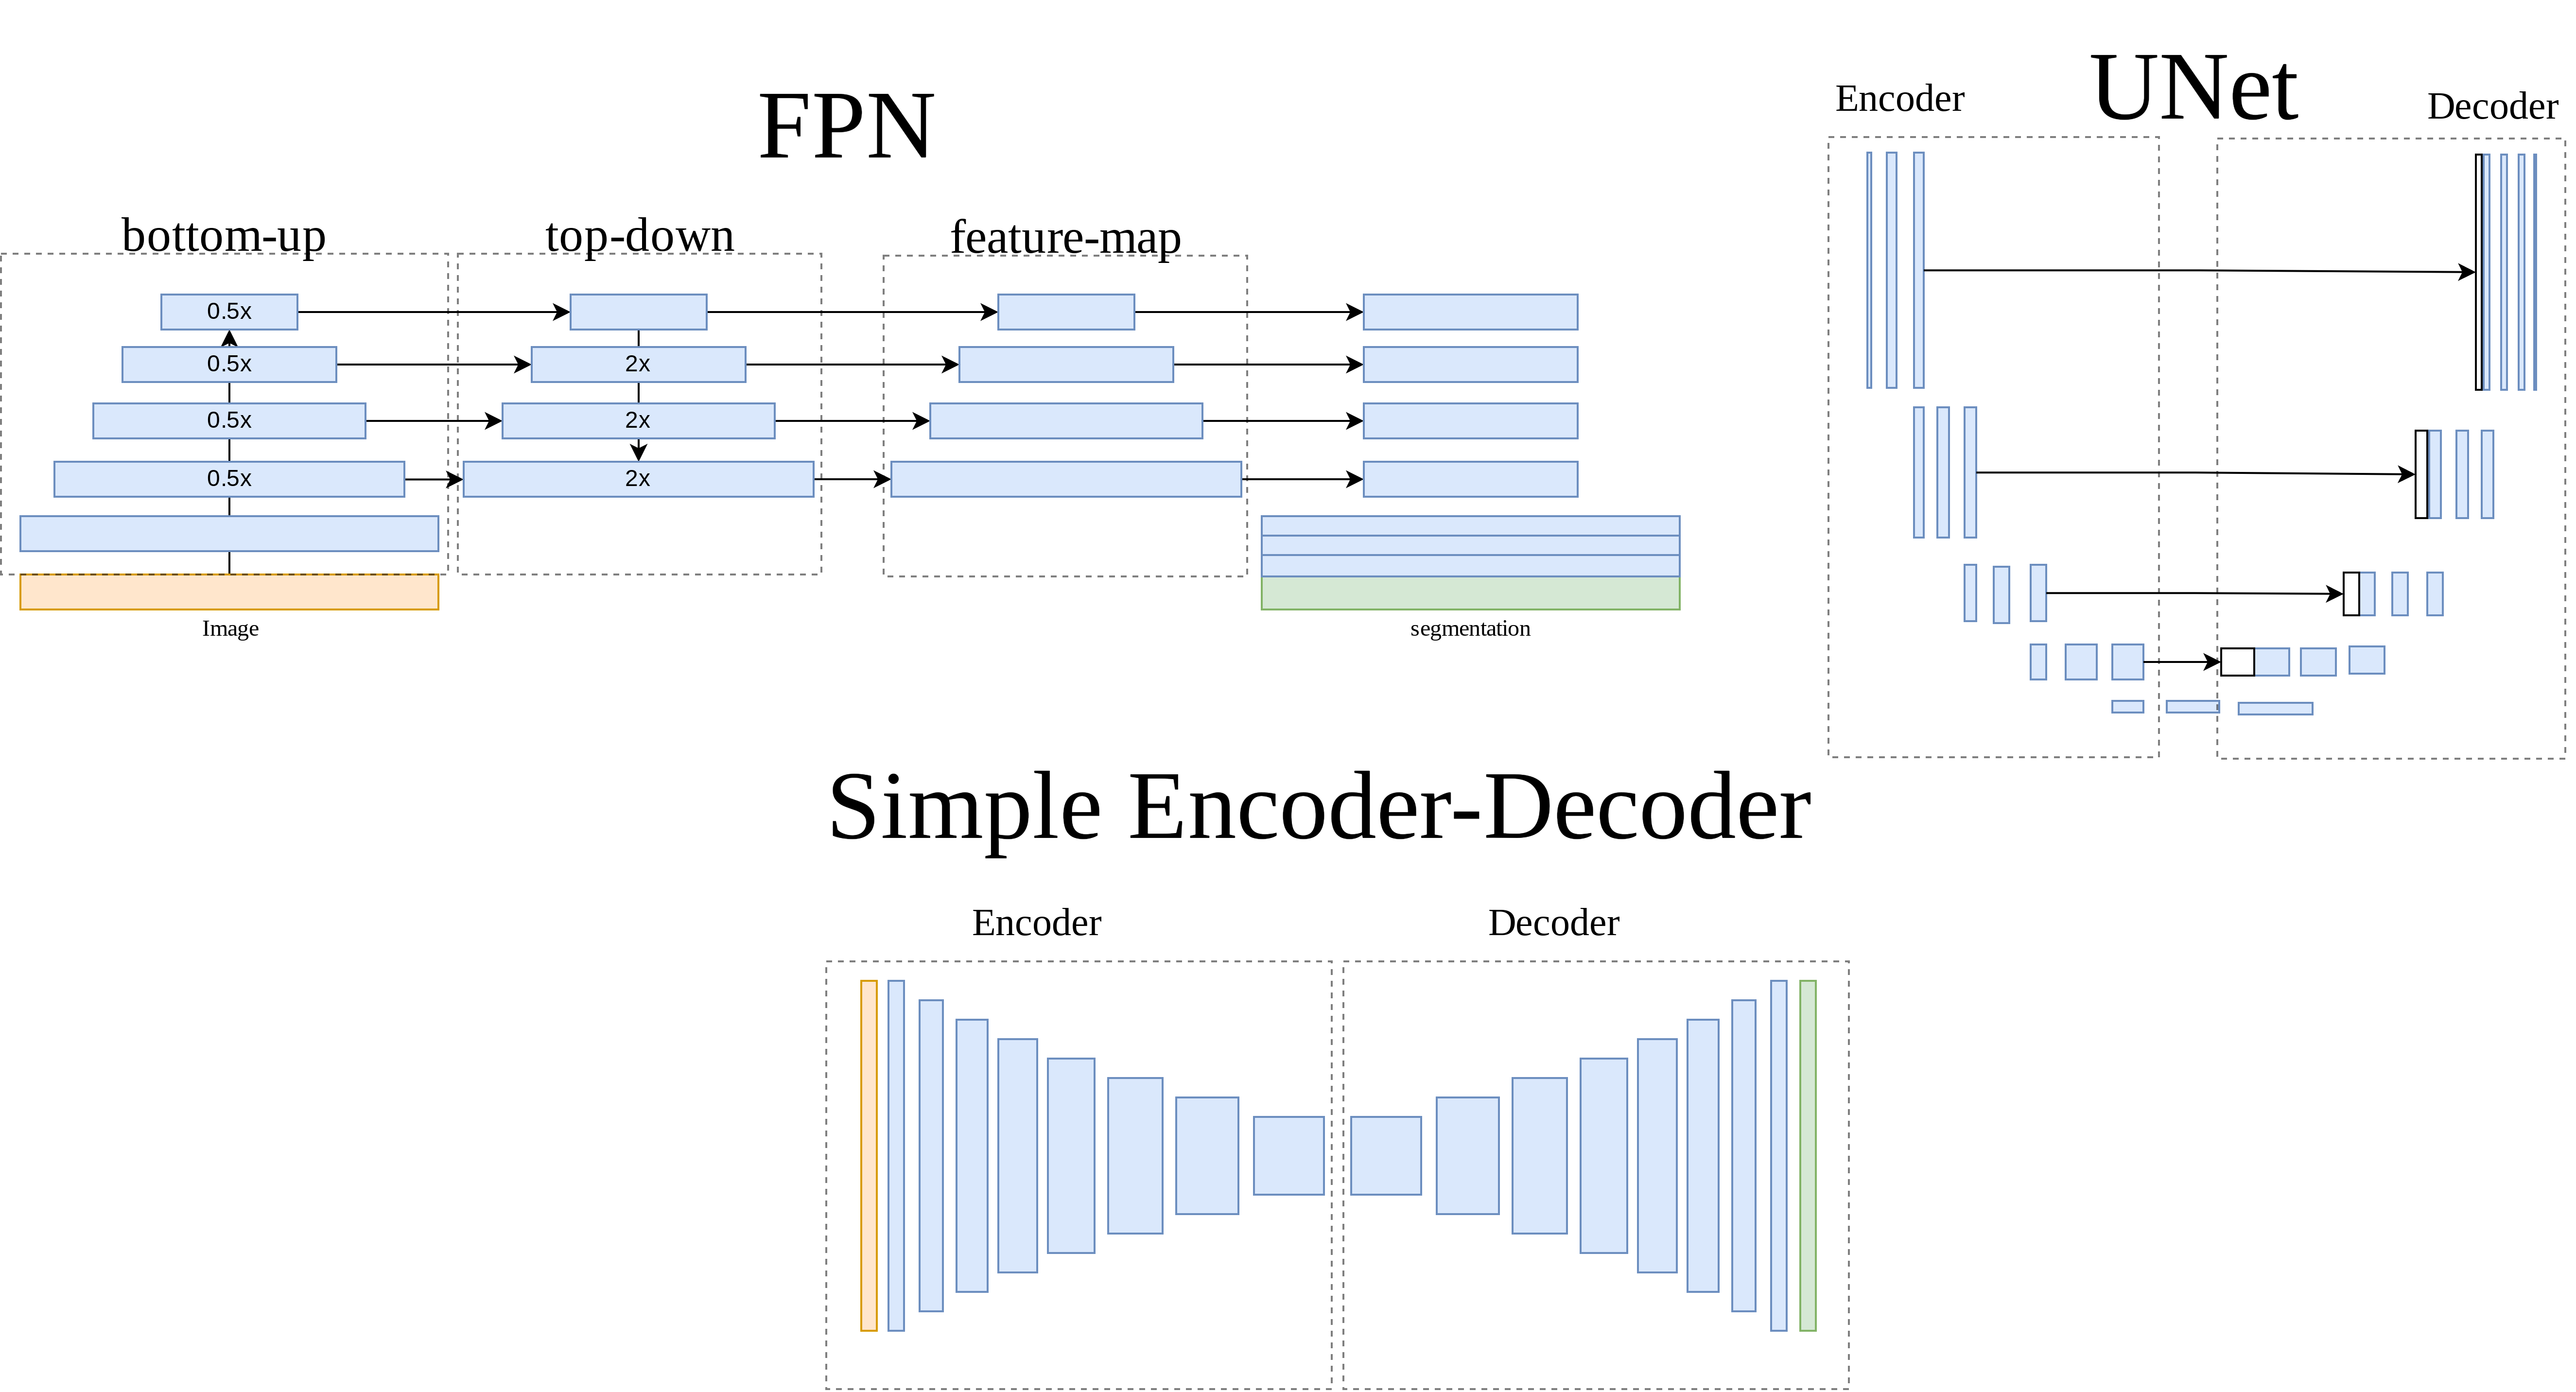
\includegraphics[width=\linewidth]{illustrations/segmentation_models.png}
        \caption{Examples of segmentation architectures}
        \label{fig:model_expl}
    \end{figure}
    
    Feature Pyramidal Networks work in a similar fashion, but instead consider the input images at multiple scales concurrently, which are then merged at the end of the network such that all scales are considered holistically.
    
    \subsection{Metrics}
        Segmentation pipelines are typically evaluated by considering the Dice Coefficient, defined in~\Cref{eq:dice}, or equivalently the \gls{iou}, defined in~\Cref{eq:iou}, between the labels and segmentation output, often along with the precision and recall. Accuracy is on its own not very informative, since high accuracies can be achieved simply by predicting all negative if the relevant objects occupy a small portion of the image.
        \begin{equation}\label{eq:iou}
            IoU(y, \hat{y}) = \frac{\sum \{y=1\}\cap\{\hat{y}=1\} }{\sum \{y=1\} \cup \{\hat{y}=1\}\}}
        \end{equation}
        \begin{equation}\label{eq:dice}
            Dice(y, \hat{y}) = \frac{2\sum \{y=1\}\cap\{\hat{y}=1\} }{\sum \{y=1\} + \sum \{\hat{y}=1\}\}}
        \end{equation}
        The \gls{iou} can to some extent be interpreted as the accuracy of the segmentation but considered only from the perspective of the regions defined by the respective segmentations, and has the advantage of facilitating easier comparison of models just accuracy.
        
        Precison and recall, defined in~\Cref{precison} and~\Cref{recall}, respectively, describe the purity and the completeness of the positive predictions. In a polyp-segmentation setting, precision describes the proportion of pixels in a segmented region that do, in fact, constitute a polyp, and recall in effect corresponds to the detection rate on a per-pixel basis. 
        
        \begin{equation} \label{precison}
            Precison = \frac{TP}{TP+FP}
        \end{equation}
        \begin{equation} \label{recall}
            Recall = \frac{TP}{TP+FN}
        \end{equation}
        
    \subsection{Losses}
    Though there are a number of different loss functions that can be used~\cite{semantic_segmentation_survey, seglosses}, it is sufficient to consider the four general types they can be categorized as:
    \begin{itemize}
        \item Distributional losses, such as cross-entropy loss. These loss functions quantify statistical properties of the label-output pairs, for instance by calculating their cross-entropy.
        
        \item Region-based losses, such as Dice-loss and Jaccard loss, which instead consider the regions defined by the segmentation labels and outputs. These are, in effect, non-thresholded and thus differentiable versions of the dice- and Jaccard-coefficients as introduced in the previous section.
        
        \item Boundary-based losses, such as boundary-loss and HD loss, which consider the boundaries of the segmentation regions.
        
        \item Hybrid losses which combine the aforementioned concepts, such as DiceCE, which as its name suggests combines Dice loss and cross-entropy loss.
    \end{itemize}
 
Asides from the use of these loss functions, model architectures, and evaluation metrics, training is otherwise fairly conventional for a deep learning pipeline. The dataloader provides an image to the model, for which the gradient is computed by descending the gradients of the loss function, with the parameters being adjusted according to the update rule defined by this gradient, the scheduler and the optimizer. 

\section{Generalization Failure in the Wild} \label{case_studies}
    Recent analyses have showed that \glspl{dnn} fail to maintain sufficient performance in deployment, even if they exhibit exceptional performance on hold-out sets~\cite{damour2020underspecification, endocv2021, shortcut_learning}. This phenomenon, which has proven to be fairly commonplace in many applications of deep learning, is known as \textit{generalization failure}. This section will cover some examples of generalization failure across different domains in order to demonstrate the pervasiveness of the problem.
    
	\subsection{Generalization Failure in Medical Imaging} \label{gen_failure_med}
	As mentioned in~\Cref{introduction}, medical deep learning pipelines are particularly prone to generalization failure due to limited dataset sizes and the sheer difficulty of the tasks involved.
	
	For example, a deep-learning based classifier which successfully detected pneumonia in X-ray scans across a number of hospitals with striking accuracy was determined to be basing its predictions not on any lesions or otherwise pathologically relevant features in the images, but rather on a hospital-specific metal token that could be found in every image, which it used in conjunction with learning the pneumonia prevalence rate of for the respective hospitals to make predictions. As a result, when deployed on data from hospitals that it had not seen during training, the system failed to generalize~\cite{pneumonia}. In another study, it was shown that a classifier intended to detect diabetic retinopathy exhibited significant variability in performance depending on the type of camera used~\cite{damour2020underspecification}. The same study also showed that similar performance variability could be found when detecting skin-conditions across demographics with differing skin tones. Finally, a model trained to detect and diagnose melanomas  was shown to in large part be basing its predictions on whether it could detect any pre-surgical markings in the vicinity of the lesion as opposed to actually learning anything about what the melanomas themselves~\cite{skin_shortcut}. As these kinds of markings naturally are highly correlated with melanomas, the model simply learned this as a shortcut. 
	
	Polyp-segmentation and detection is also, naturally, a victim of generalization failure, as evidenced by EndoCV2021~\cite{endocv2021}. Even the best-performing models exhibited considerable performance degradation when evaluated on unseen datasets, collected from separate centers than the training data. 
	 
	\subsection{Generalization Failure in General}
	Though generalization failure is perhaps best represented in medical domains, the phenomenon is pervasive in practically every application of deep learning, albeit to varying degrees. It has for instance been shown that CNNs trained on ImageNet, one of the largest and most diverse datasets in the domain of computer vision, are heavily biased towards textural features, and consequently fail when the texture of the input is modified, despite the shape and structure of the relevant object remaining recognizable~\cite{texturebias}. Though this result is based on evaluation on synthetic data, it highlights a key property of deep learning pipelines: namely that they do not necessarily learn features that are causal - in other words, that they are intrinsic to the relevant object - inasmuch as they learn features that are highly correlated with it- in other words, features that are associated with the object but are not intrinsic to it. Though the texture of cat fur for instance is highly correlated with the "cat" class, it is not the fur that makes the cat. In Figure \ref{cat_elephant}, for instance, it is clear that image (c) should be classified as a cat more than an elephant. Granted, this example is as mentioned synthetic, but a similar situation could arise if the classifier for instance was tested on a black-and-white image of a hairless cat. 
	\begin{figure}[htb]
		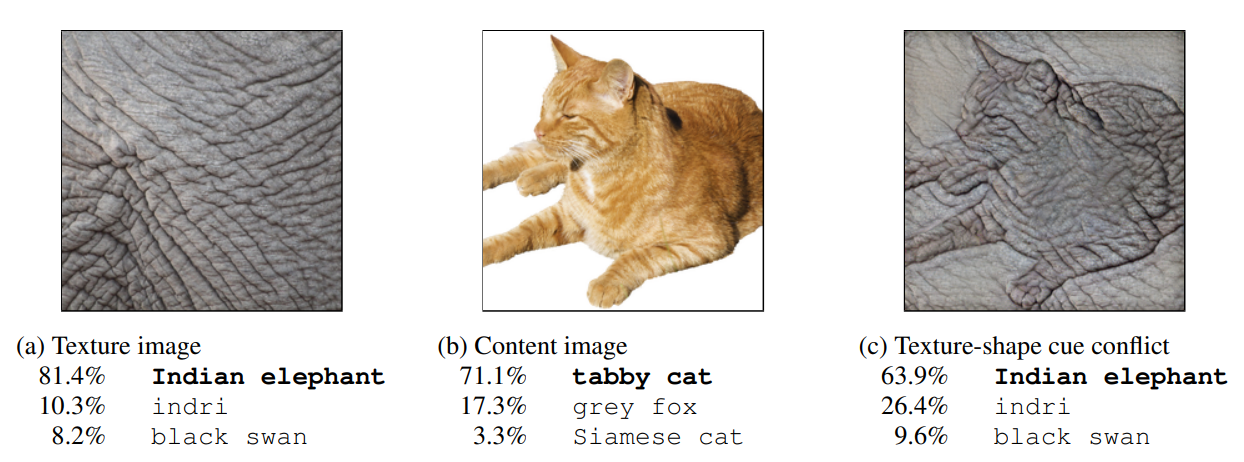
\includegraphics[width=\linewidth]{illustrations/cat_elephant.png}
		\caption{Classifiers trained on ImageNet are biased towards textural features. Adapted from \cite{texturebias}.}
		\label{cat_elephant}
	\end{figure}
	
	This behaviour of considering correlations over causation can also be found in state-of-the-art image captioning systems, for instance Microsoft Azure's computer vision API and NeuralTalk2~\cite{electric_sheep}, wherein the model seemingly hallucinates that it sees sheep when evaluated on images of grassy pastures or hills. This is shown in~\Cref{sheep}. Once again, it is of course natural to expect that sheep can be found in these contexts, but it is not these contexts that define what it means to be a sheep. Grassy pastures and sheep are not causally related, only correlated, but deep learning pipelines lack the nuance required to understand this fact. 
	\begin{figure}[htb]
		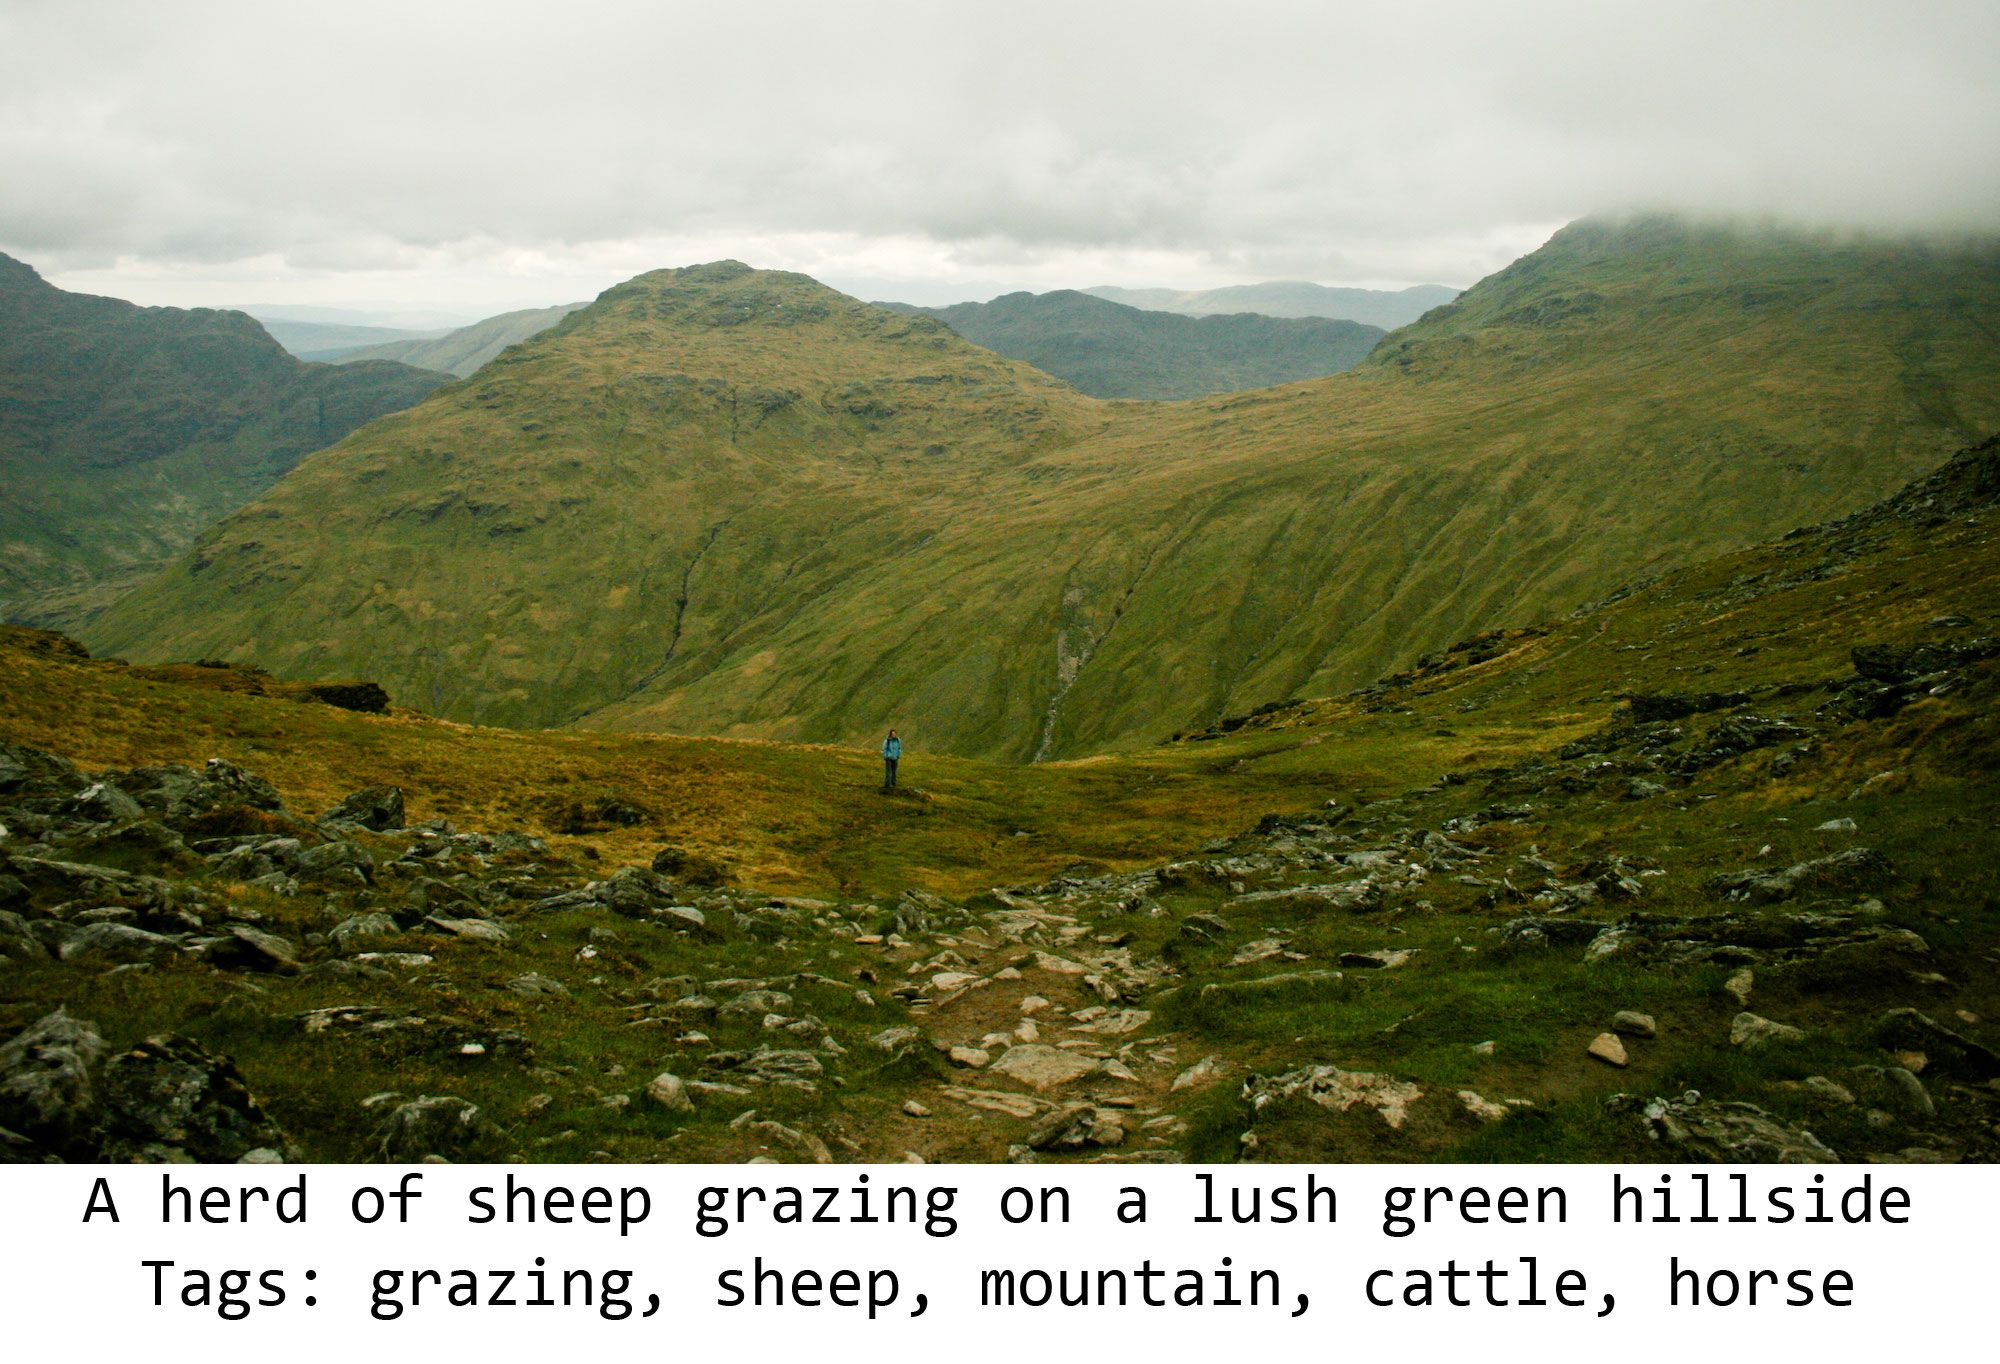
\includegraphics[width=\linewidth]{illustrations/sheep.jpg}
		\caption[Deep Hallucination]{Deep captioning models hallucinate sheep (and other animals) when presented with contexts highly correlated with sheep. Adapted from~\cite{electric_sheep}}
		\label{sheep}
	\end{figure}

	Another characteristic of deep learning that supports this argument is the effectiveness of adversarial attacks~\cite{adversarial_bugs_features}, which specifically target weaknesses in the representations used by a given \gls{dnn} through any number of means in an attempt to induce high rates of incorrect, yet highly confident predictions. Gradient-based adversarial attacks, for instance, use the gradients of the model to break even the most sophisticated and well-trained pipelines merely by adding some carefully crafted, yet visually imperceptible noise to the inputs~\cite{adversarial_attacks}. Even without access to the gradients, there exists a multitude of so-called black-box attacks that only use output samples to generate similarly effective attacks~\cite{blackbox_adv}. Finally, it has been shown that adding minor visual distractions to objects, for example adding bits of tape or graffiti to stop signs, dramatically increases misclassification rates~\cite{physical_attacks}. 
	
\section{Generalizability Theory} \label{gen_theory}
	Exactly why and how \glspl{dnn} seem to so persistently fail to generalize is a topic of ongoing research, and the available literature seems to suggest that the problem is multifaceted. This section summarizes and distill the findings and analyses performed in the literature so far. It will cover the theoretical basis of generalization and why one might expect \glspl{dnn} to generalize, discuss the key characteristics of generalization failure, and finally discuss why and how these characteristics arise with respect to the theory.
	
	\subsection{Generalization through Empirical Risk Minimization} 
		Naturally, deep learning would not be as ubiquitous as it is if there was not some semblance of an expectation that their striking performance was generalizable and performant also outside the idealized settings typically involved in research. The theoretical basis that informs this belief in (most) modern deep learning pipelines is the idea of so-called \glsfirst{erm}, wherein it is assumed that the dataset upon which the model is trained is a representative sample of the distribution of all possible samples in the relevant domain. In other words, it assumes that the dataset is \gls{iid} to the domain distribution. To better understand this assumption, it is beneficial to consider it from first principles: 
		
		At the most fundamental level, the goal of machine learning is to learn a mapping between two spaces of objects \(X\) and \(Y\). This mapping, namely the function \(f: X \rightarrow Y\), maps some input object \(x \in X\), an image for example, to a corresponding and application-relevant output object \(y \in Y\), for instance a segmentation mask or class-wise probabilities. It is worth noting, however, that \(f\) is not as much a function in the mathematical sense as much as it is an abstraction of the relationship that the deep learning system is intended to capture. \(f\) cannot as a consequence typically be modelled explicitly. Instead, machine learning systems aim to find a sufficient approximation of this mapping by leveraging a training set \(\{x_i, y_i\}_{0...n}\). This is referred to as \textit{supervised learning}, and the resulting approximation found using the training set is denoted by \(h: X \rightarrow \hat{Y}\), and typically referred to as the \textit{hypothesis}.  
		To find such an approximation, it is assumed that there exists a joint probability distribution over \(X\) and \(Y\), namely \(P(x,y)\), and that the training data \(\{x_i, y_i\}_{0...n}\) is drawn from this probability distribution such that the resulting sample distribution is independent and identically distributed to \(P(x,y)\). This is the aforementioned \gls{iid} assumption. By modelling the mapping as a joint probability distribution, one can model uncertainty in the predictions by expressing the output as a conditional probability \(P(y|x)\). In conjunction with a loss-function \(L(h(x),y)\) which measures the discrepancy between the hypothesis and the ground truth, these assumptions allows us to quantify the expected performance of a given hypothesis:
		\begin{equation}
		    R(h) = \mathbb{E}[L(h(x),y)] = \int L(h(x),y) dP(x,y)
		\end{equation}
		Using this framework, one can then find an \gls{iid}-optimal hypothesis, often called a \textit{predictor}, by finding the predictor \(h^*\) among a fixed class of functions (defined by network architecture) \(\mathcal{H}\) that minimizes risk:
		\begin{equation}
		h^* = \argmin_{h \in \mathcal{H}}R(h)
		\end{equation}
		
		Since \(P(x,y\)) is not known, however, one cannot compute \(R(h)\) explicitly. Instead, the expected risk has to be estimated empirically, i.e by finding the arithmetic average of the risk associated with each prediction by the hypothesis over the training set:
		\begin{equation}
		R_{emp}(h) = \frac{1}{n}\sum_{i=1}^{n}L(h(x_i), y_i)
		\end{equation}
		This risk can in turn be minimized with respect to the hypothesis class. This is called empirical risk minimization (\gls{erm}):
		\begin{equation}
		\hat{h} = \argmin_{h \in \mathcal{H}}R_{emp}(h)
		\end{equation}
		To reiterate, the central idea with this approach to machine learning is that the training data can be considered a finite \gls{iid} sampling of the underlying distribution. As such, by the central limit theorem, the hold-out performance of the computed hypothesis will approach \gls{iid}-optimal performance given a sufficient amount of training data and some sufficiently capable training procedure. This should in theory allow deep learning systems to be able to generalize, since the empirical risk in theory can approximate the true risk arbitrarily well given sufficient training data.

		As described in section \ref{case_studies}, \gls{erm} nonetheless readily fails to generate generalizable predictors with respect to out-of-distribution data. There are multiple dimensions to this phenomenon, as there are several means by which a model can fail to generalize. To better understand these failure modes, it helps to consider the assumptions that are made in the formulation of \gls{erm}, namely that:
		\begin{enumerate}
			\item \(f\) exists in \(\mathcal{H}\) \label{underfit}
			\item The optimal predictor can be found solely through minimizing \(R_{emp}(h)\)\label{overfit}
			\item \(\{x_i, y_i\}\) is an \gls{iid} sampling of \(P(x,y)\) \label{structural_misalignment}
			\item \(\hat{h}^*\) is unique in \(\mathcal{H}\)\label{underspecification}
		\end{enumerate}
		As the following sections will show, violations of any one of these assumptions can and typically will result in generalization failure. 

	\subsection{Realizability and Underfitting}
		Violations of assumption \ref{underfit} corresponds to a well known and fairly well understood form of generalization failure, namely underfitting. One can however argue that underfitting can be all but discounted as plausible explanation for the pervasiveness of generalization failure observed in modern deep learning pipelines. Underfitting occurs when the model simply lacks the complexity required to encapsulate the patterns necessary to form generalizable interpretations of the data. To give a simple example - consider the problem of trying to fit a linear model to the following dataset: 
		\begin{figure}[htb]
			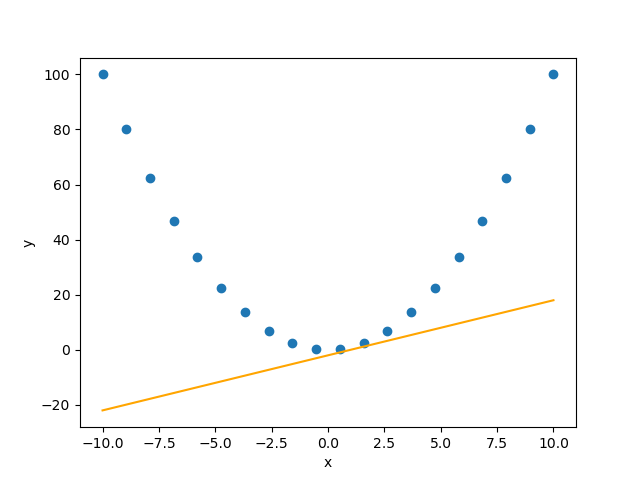
\includegraphics[width=\linewidth]{illustrations/regression_example.png}
			\caption[Underfitting]{A linear model cannot fit polynomial data}
			\label{underfit_example}
		\end{figure}
		Obviously, no amount of optimization of the parameters in the linear model can ever result in a sufficient description of the underlying data and the function it follows, namely \(y=x^2\). 
		
		This, however, does not necessarily mean that an underfitted model cannot perform well; the data shown in~\Cref{underfit_example} function is after all locally linear, and if it is only evaluated on a limited region, a linear model may perform just fine. One can as such argue that \glspl{dnn} in turn may be underfitting, and that generalization failure analogously corresponds to evaluating on data outside of this locally linear region. This, however, is unlikely to be the case, as evidenced by recent results in the study of model complexity.
		
		Modern \glspl{dnn}, as it turns out, have practically infinite so-called effective capacity - i.e, they can model more or less arbitrarily complex data. It can for instance be shown that even a 2-layer feedforward neural network is capable of fitting noise to random labels with 100\% accuracy~\cite{randomlabels}. Consequently, it is fairly reasonable to expect that the hypothesis space of the highly complex models used today contains a generalizable predictor and thus that assumption \ref{underfit} holds. In the literature, this is often referred to as the realizability assumption~\cite{machine_learning_theory}. 
		
	\subsection{Overfitting, Inductive biases and training}
	The high effective capacity of \glspl{dnn} does, however, result in a number of side-effects that actually hamper generalization. Though this capacity does suggest that most learning problems are realizable, the problem of finding a generalizable predictor from the hypothesis space is nevertheless not at all trivial. \gls{erm} presupposes assumption \ref{overfit} - i.e that there exists some way to precisely find the risk-minimizing predictor \(\hat{h} = \argmin_{h \in \mathcal{H}}R_{emp}(h)\), and as such that there is some ideal optimization procedure that can be leveraged to this end. This, of course, is not the case. Instead, a search of the hypothesis-space is performed using gradient-descent. On its own, this search is not necessarily guaranteed - or for that matter even likely - to find an \gls{iid}-optimal predictor. This is due to the inherent nature of the search space - \glspl{dnn} have parameter counts numbering in the millions or more, and try to determine optimal parameter configurations from comparatively miniscule datasets.
		
	Without certain precautions, this may result in the pipeline returning predictors that in effect simply memorize the training data, without learning anything useful about the domain itself. This is referred to as overfitting~\cite{deep_learning_book}. 

	Memorizing all the training data is, however, risk-minimizing. To illustrate, consider a predictor which simply memorizes the segmentation masks for the polyps in a given dataset, and simply returns the corresponding mask when given an image it has trained on, and returns a zero-mask otherwise. This, as explained earlier in this section, is entirely within the capabilities of \glspl{dnn} due to their high effective capacity. When evaluating this predictor on the dataset upon which is was trained, the empirical risk will naturally be zero, since it will correctly return the right segmentation for a given image despite not having learned anything useful about polyps whatsoever, or for that matter anything useful about images.

	Thus, certain constraints have to be imposed on the search space to avoid overfitting. These constraints have to be defined a-priori, and are often referred to as the \textit{ inductive biases} of the pipeline. 

	This is often achieved through the use of regularization techniques. Dropout~\cite{dropout}, for instance, biases the model towards learning representations that distribute well across the network and can work independently of one another. Weight decay~\cite{weight_decay} biases the model toward low-magnitude parameters, and thus simpler representations. Data augmentation biases the model towards learning features that hold across augmented samples, and so on.

	Besides regularization, certain inductive biases can also be imposed through modifying the training routines themselves, by for instance pretraining~\cite{pretrain}, contrastive representation learning~\cite{contrastive} or multi-task learning~\cite{ddanet, multitask}, etc.

	Determining the effectiveness of these techniques and tuning the hyperparameters that inevitably arise naturally requires a specific evaluation procedure~\cite{deep_learning_book}. To this end, most deep learning pipelines leverage hold-out sets, wherein the data is partitioned into three folds - the training set, used to compute gradients and train the model, the validation set, used to tune hyperparameters, and a test-set, used to evaluate the \gls{iid} generalizability of the resulting predictor. More sophisticated methods, such as cross-validation, are also often used. 

	Fundamentally, each of these techniques increase generalization by limiting the search space, in effect redefining \(\mathcal{H}\). The more inductive biases are imposed onto the model, the smaller \(\mathcal{H}\) in effect will be. 

	Modern Deep learning pipelines regularly employ several of these techniques, often in conjunction with one another, and consequently easily avoid overfitting and achieve good results on the test-set. This only guarantees \gls{iid} generalization, however, and thus these models still readily fail to generalize to OOD data. This is illustrated in~\Cref{fig:feature_types} That is not to say that regularization and other ways of imposing inductive biases on the model does not aid in generalization, only that overfitting does not explain the pervasiveness of generalization failure that can be seen today. 
	\begin{figure}
	    \centering
	    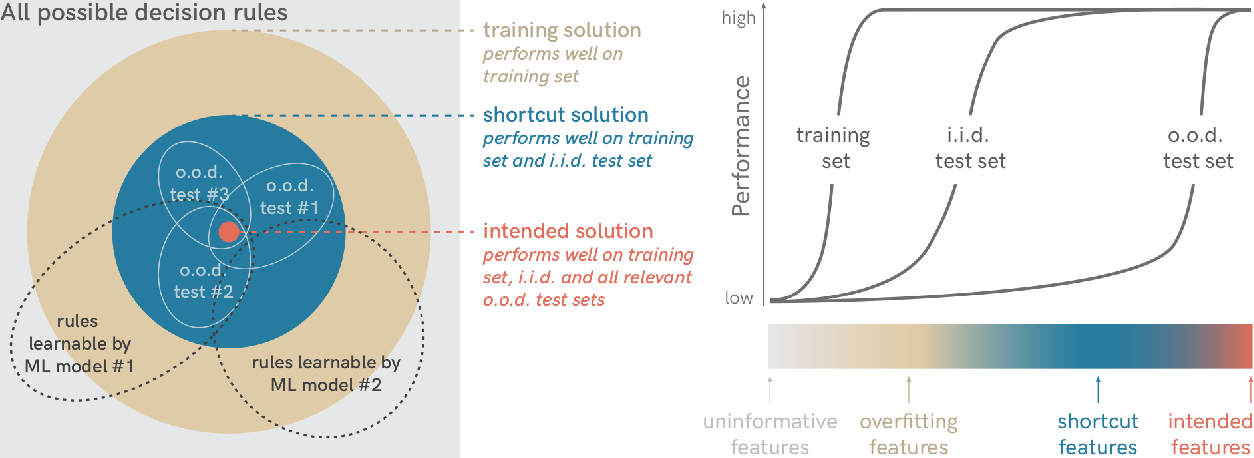
\includegraphics[width=\linewidth]{illustrations/features.png}
	    \caption[Feature Taxonomy]{Good performance on unseen IID test sets do not guarantee generalization, as it only requires learning IID-biased features. Generalizable performance, naturally, requires generalizable features. Adapted from~\cite{shortcut_learning}}
	    \label{fig:feature_types}
	\end{figure}

	\subsection{Structural Misalignment and dataset bias}
	Recent research on generalization failure often attributes it to a structural misalignment between the predictor as generated by \gls{erm} and the causal structure which it ideally should encode~\cite{adversarial_bugs_features,shortcut_learning,IRM, causality}. Generally, this misalignment occurs as a result of the predictor learning spurious or otherwise causally unrepresentative features that nonetheless perform well within the training distribution. This if of course made evident as soon as the predictor is exposed to any form of distributional shift, at which point it will fail to generalize. These distributional shifts can range in magnitude, from changes in imaging modalities, common corruptions such as noise or blurs~\cite{corruption_robustness} or spatial transforms~\cite{spatial_robustness} to practically imperceptible perturbations, typically exemplified by adversarial attacks~\cite{adversarial_attacks}. \gls{erm} does not and cannot guarantee invariance to distributional shifts, as it assumes that the training data is \gls{iid} to \(P(x,y)\). This is not, however, necessarily as much of a flaw with \gls{erm} inasmuch as it is a flaw in the reasoning behind our expectations. 
		
	To illustrate, consider the rather pertinent example of training a model exclusively on either white-light or narrow-band endoscopy. Assume that there are two datasets, each containing samples depicting identical scenes, with the only difference being that dataset A employs white-light endoscopy, whereas dataset B employs narrow-band endoscopy. Ideally, a model trained on either dataset should generate predictors that can generalize to the other, and though one may be optimistic and hope this is the case, this is in no way guaranteed. The causal structure behind the decisions - i.e what exactly makes a polyp a polyp - is never considered at any point in the training process. Instead, the models will simply try to leverage whatever predictive patterns can be found the training data. The model trained on narrow-band images may for instance principally consider the textural characteristics of the polyps, which narrow-band endoscopy enhances. Conversely, the model trained on white-light images, lacking access to these textural characteristics, may instead consider more color- or shape-based features. Naturally, if this narrow-band-texture-biased model is deployed in white-light endoscopy, it is not likely to succeed since its principal discriminative features no longer are particularly useful. Similarly, the colour-biased model would fail when deployed in narrowband endoscopy since the colours it once used to distinguish polyps are no longer predictive in narrowband images.  

	\begin{figure}[htb]
		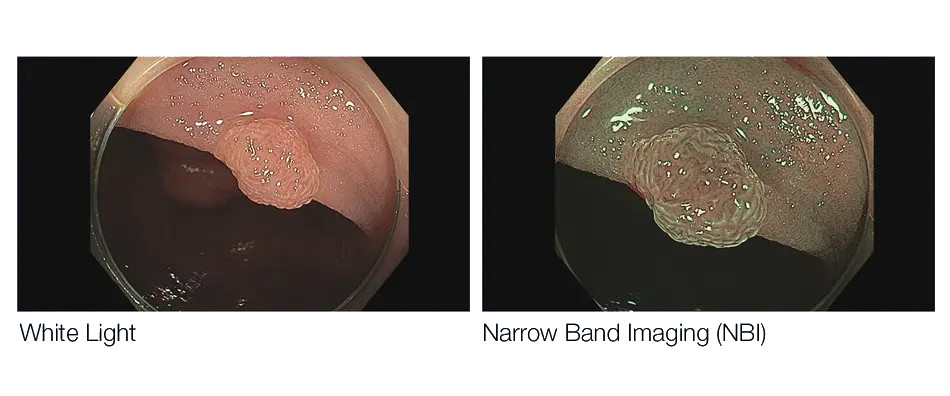
\includegraphics[width=\linewidth]{illustrations/narrow_band.jpg}
		\caption[NBI v White-light imaging]{Narrowband imaging and white-light endoscopy constitutes a distributional shift. Adapted from~\cite{nbi_img}}
		\label{imaging_modalities}
	\end{figure}

	Though the features each model learns are not particularly representative of the broader context of what makes a polyp a polyp, they make sense when considered from the perspective of either of the two modalities. When considering only narrow-band imaging, it makes some sense to heavily weigh the texture of the polyps. When considering only white-light imaging, it makes some sense to heavily weight the shape and color of the polyps. Though humans are capable of appreciating broader context and subconsciously know that certain features are ancillary rather than causal (and perhaps more importantly: know the strengths and weaknesses of each modality), \glspl{dnn} lack the inductive biases needed to take this into account. Once again, \glspl{dnn} merely leverage the first and best predictive patterns found during the training process, and cannot be expected to optimize for specific invariances on their own, irrespective of how self-evident these invariances may be for humans. This predilection towards dataset-specific features is aptly referred to as dataset bias. 
	
	\subsubsection{Shortcut Learning}
	In the aforementioned example, though the features each predictor learns is not robust to dataset shift, they nevertheless have causal explanations. The causal structure that they correspond to is of course not dataset-agnostic, and as a result flawed in their own way, but the patterns the respective models leverage to interpret the data are not particularly irrational. As it turns out, however, \glspl{cnn} are unlikely to learn such causally viable features in the first place. In other words, the predictors would not necessarily learn to consider texture in narrow-band images - it could learn any arbitrary pattern so long as it is predictive. Moreover, if such interpretable distributional shifts were the principal cause of generalization failure, generalizability could be practically guaranteed by explicitly modelling the effects such shifts induce and taking this into account in the pipeline. In the aforementioned example, one could for instance train some model to map from one lighting environment to the other. Though this would imbue the model with an inherent invariance to the choice of lighting, it is nonetheless not given that the resulting model will be perfectly generalizable.

	Consequently, though these detectable forms of distributional shifts also hold some importance when designing generalizable models, a more pervasive and substantially more significant issue is the fact that many of the distributional shifts encountered in clinical settings are not necessarily considered significant or for that matter at all perceptible to a human observer. A human would for instance not be significantly affected by slightly noisy, blurry, rotated, or compressed images, nor would they in all likelihood notice these perturbations. \glspl{dnn}, on the other hand, have been shown to be highly sensitive to these and several other forms of minor perturbations~\cite{noise_robustness, corruption_robustness,adversarial_training}. Moreover, a human would likely not pick up on subtle phenotypic cues that may exist in the colon during endoscopy, whereas a \gls{dnn} may leverage some of these cues to inform their decisions, and hence exhibit varying performance across different demographics. 

	It is important to note, however, that despite how these two forms of distributional shift may at surface level appear as completely separate classes of problems, they can both be traced to the same phenomena - namely that \glspl{dnn} do not leverage any form of causal logic to inform their decisions and, as mentioned previously, simply exploit any sufficiently predictive pattern they may observe in the data. This phenomenon has been shown to be pervasive across all manner of domains, from natural language processing~\cite{dl_nlp} and computer vision to reinforcement learning~\cite{computer_vision} and algorithmic decision-making\cite{dl_recommend}. This is referred to as shortcut learning~\cite{shortcut_learning} or the Clever Hans effect~\cite{cleverhans}. 

	Shortcut learning and the use of the brittle features that often constitutes the shortcuts has also been identified as one of the key properties that explains the effectiveness and pervasiveness of adversarial attacks~\cite{adversarial_bugs_features}. Naturally, a generalizable predictor should be robust to such minor perturbations, as the model should not in the first place be learning features that get perturbed to any significant degree by adding such high-frequency, low-amplitude noise. Adversarial attacks simply leverage the high degrees of sensitivity inherent to shortcut features, and construct perturbations according the direction in the search space that corresponds to the principal component of this sensitivity~\cite{sensitivity}. 

	\subsection{Underspecification}
	Closely related to shortcut learning is underspecification~\cite{damour2020underspecification}. A machine learning pipeline can be considered underspecified when it can return any number of risk-equivalent predictors when evaluated on an \gls{iid} holdout set, dependent only on the random variables used within the training procedure - i.e dropout, seed initialization, and so on. Even with identical hyperparameters, a given training procedure can return any number of predictors each having learned different patterns. One predictor may have learned one shortcut, another may have learned a different shortcut, and one may have fully learned the actual causal relationships it is intended to. With \gls{erm}, and in particular with \gls{ind}-oriented evaluation procedures, these are all erroneously considered equivalent. 

	Note that this does not however presuppose anything about the relative occurrence rates of generalizable and non-generalizable predictors. It may not necessarily even be the case that the pipeline can return a generalizable predictor at all. Only that there exists a multitude of risk-equivalent predictors in the search space the optimizer typically explores. Nor does it presuppose anything about the distribution of predictors, only that there is indeed a distribution. 

	This is evidenced by the fact that generalizability can vary greatly depending on the choice of random seed used during training. In the foundational paper on underspecification in deep learning, for instance, it was highlighted that certain classification pipelines can produce predictors that vary in ood accuracy by up to 10\%~\cite{damour2020underspecification}. This is a function of the robustness of the learned features and how likely the pipeline is to return the corresponding predictors. 
	
	\subsection{A probabilistic perspective of generalization} \label{probpersp}
	As established, modern deep learning pipelines are not capable of reliably returning generalizable predictors. However, they are not necessarily precluded from it. One can to some extent model this probabilistically by considering the distribution of parameters given the training data, \(p(w | \mathcal{D})\). Though it is impossible to know which part of this distribution corresponds to generalizable predictors, it has been shown that marginalizing over this distribution increases generalizability~\cite{bayesian_generalization,endoensemble,divergentnets,ensemble_machinereading}. This is referred to as Bayesian Learning~\cite{bayesian_case}. The details and statistical nuances behind this is somewhat outside of the scope of this thesis, so for now it is sufficient to simply consider it as a way to account for some of the variability inherent to the distribution of predictors that can be generated by a deep learning pipeline. 

	This view can be more readily understood by taking a probabilistic perspective of generalization as a whole~\cite{bayesian_generalization}. Generalizability can be considered as a two-dimensional quantity, consisting of the support and inductive biases of a model. The inductive biases are as mentioned the constraints by which the model learns, ranging from model-construction - e.g positional invariance in CNNs - to regularization - e.g dropout, data augmentation, etc - and specific training routines - i.e multitask learning, contrastive representation learning, etc. The support, on the other hand, describes the ability of the model to encode certain decision rules. Ideally. support should be maximized, as this permits a given model to learn arbitrarily complicated decision rules. Similarly the amount of inductive biases imposed on the model a-priori should also be maximized, as it reduces the probability of learning decision rules that, though predictive, are not causally related to the problem. 

\section{Related work on Generalizable Deep Learning}
To summarize the preceding sections, generalization failure occurs due to the weaknesses inherent to \gls{erm}. The features that \gls{erm} learn to incorporate are often spurious, and the pipeline can return any number of spurious or non-spurious predictors from identical training procedures up to choice of random seeds. The approaches that have exhibited the highest degrees of success towards increasing generalization as a consequence tend to address these issues in some way or another. This section will discuss a number of such methods, including data-augmentation, model-debiasing, alternative learning paradigms, and ensemble learning.

\subsection{Data-augmentation}
One of the most well-studied approaches to increasing generalizability is the use of data augmentation. Data augmentation is typically
implemented in deep learning pipelines in order to prevent overfitting, often in conjunction with other regularization methods. As discussed earlier, overfitting constitutes generalizability failure in its own right, but augmentation has also been shown to have positive effects for out-of-distribution generalization. It has for instance been shown that carefully designing augmentation procedures increases the generalizability of polyp segmentation models~\cite{polyp_augmentation} and prostate segmentation models~\cite{augmentation_prostate}. 

This can be readily explained by considering the perspective mentioned in Section \ref{probpersp}. In effect, data augmentation is simply a method to increase the model's support, and can be shown to have comparable effects to adding a second dataset source~\cite{generalization_datamod}. This is because the empirical risk will be best minimized by leveraging features that are conducive to minimizing risk across both the augmented data and unaugmented data (though as will be discussed in~\Cref{methods}, they are not necessarily equally weighed). 

Moreover, the choice of augmentations that are used can to some extent be considered as adding additional inductive biases to the pipeline, which as established increases the likelihood of learning generalizable features. For instance, by augmenting with random rotations, rotational invariance is presupposed. By augmenting with color jitter, invariance to global color-transforms is presupposed.  By employing additive noise, invariance to additive noise is presupposed, and so on. From an \gls{erm} perspective, this can also be thought of as improving the empirical risk estimate. 

\subsection{GANs, VAEs and Distributional Modelling}

There has also been a large body of work dedicated to leveraging recent advances in generative models such as \glspl{gan} and \glspl{vae} to serve as synthetic data augmentation. These types of approaches have also been shown to increase generalizability in CT segmentation~\cite{cyclegan} and x-ray based detection of covid-19~\cite{covid}. To understand why this is the case, and the methods proposed in~\Cref{methods} leverage a form of \gls{gan}, it is worth explaining how these networks work in further depth.
    \subsubsection{Generative Adversarial Networks}
     \glspl{gan} are very simply put a type of deep learning framework intended to be able to replicate the distribution upon which they are trained. A \gls{gan} trained on images of human faces, for instance, can in theory generate a practically infinite number of novel, believable human faces. This is examplified in~\cite{facegan}. 
     
     \glspl{gan} achieve this through a particular training regiment, wherein two models - the generator and the discriminator - contest one another in a zero-sum game. The generator, as its name suggests, attempts to fool the discriminator by generating synthetic data from noise, intended to be indistinguishable from what one might expect a sample from the training data to look like. The discriminator, on the other hand, tries to classify an incoming image as synthetic or not. This is illustrated in~\Cref{fig:gan} 
     \begin{figure}
         \centering
         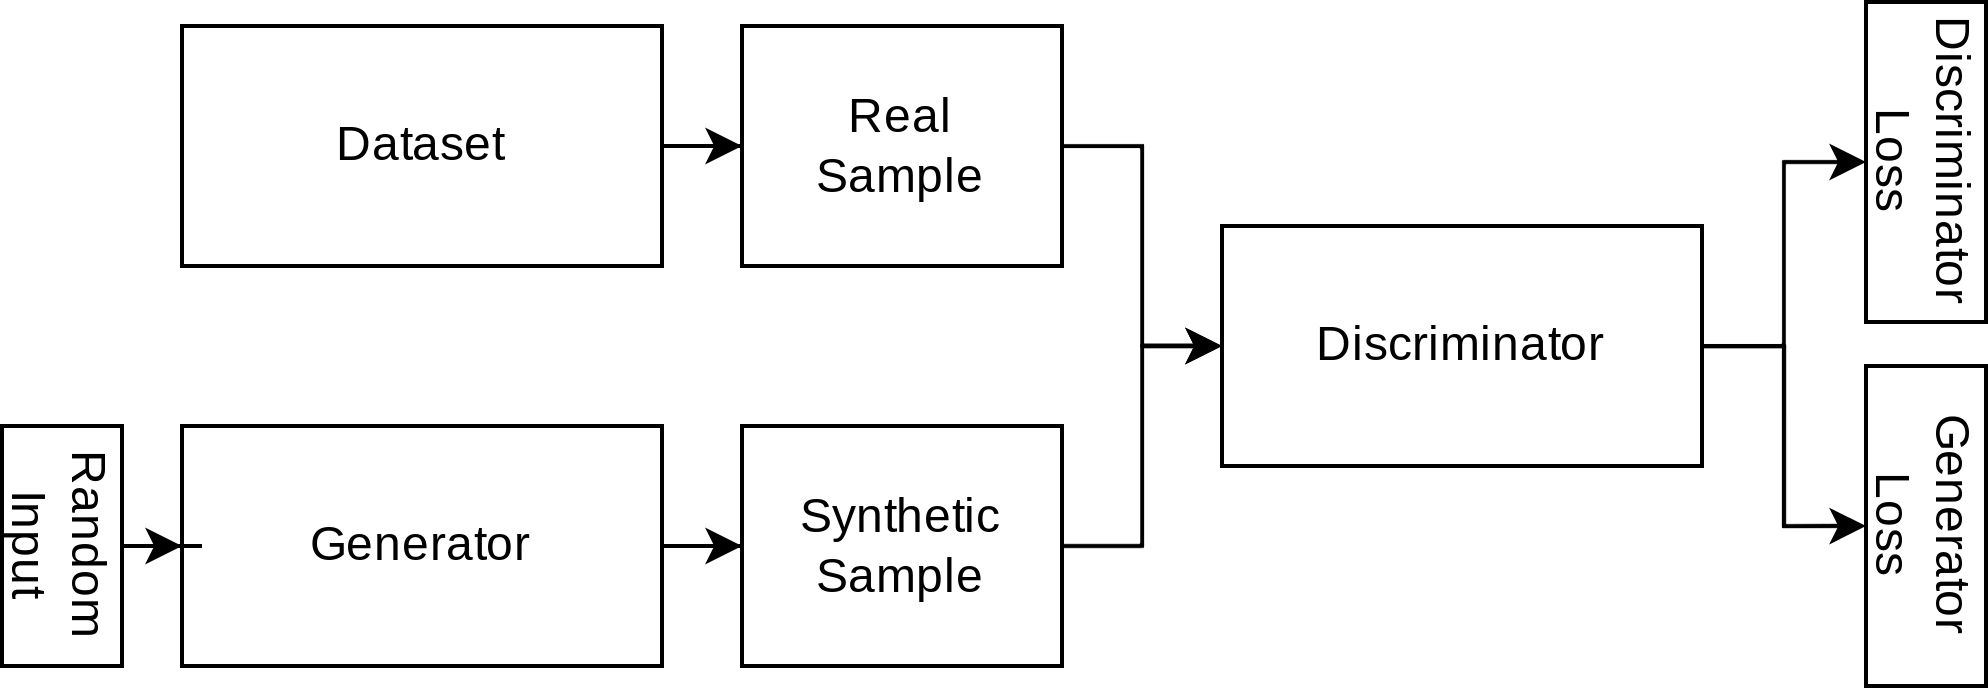
\includegraphics[width=\linewidth]{illustrations/gan.png}
         \caption{Generative Adversarial Network Framework}
         \label{fig:gan}
     \end{figure}
     
     This is achieved by training the generator and discriminator in an interleaved fashion, wherein the gradient updates for each model are a function of the output of the adversary. To illustrate, consider the GAN pipeline as introduced in~\cite{gan_first}:
     Let \(G(\cdot)\) be the generator, and \(D(\cdot)\) be the discriminator. Let \(x\) be a training input sample, and \(z\) be random noise. The generator will then try to minimize the following quantity, whereas the discriminator will try to maximize it:
     \begin{equation}\label{gan_loss}
        \mathcal{L}_G = \log{D(x)} + \log{(1-D(G(z))} 
     \end{equation}
     This way, when the generator is being trained, it learns to generate outputs that fool the discriminator. This corresponds to the discriminator outputting a high probability of the image being real, i.e \(D(G(z)) = 1\). Conversely, when the discriminator is being trained, it learns to generate outputs that correctly classify the generated samples as fake, i.e \(D(G(z)) = 0\), and the real samples as real, i.e \(D(x) = 0\). 
     
     \subsubsection{GANs, Generalization and Modelling the Distribution}
     Ideally, the fully trained generator should be capable of generating the full space of images defined by the training distribution \(\mathcal{X}\) simply by modulating the input vector. And indeed, mathematical analysis shows that GANs are capable of approximating this distribution arbitrarily close given infinitely sized datasets, infinite training time and infinite model support~\cite{gan_first}. 
     
     Whether this is the case in practice is a matter of ongoing research, however, with mathematical analyses suggesting that sufficient approximation of the distribution is impossible without the aforementioned assumptions~\cite{gan_learning_distribution}.
     
     This is evidenced by the pervasiveness of a phenomenon referred to as mode-collapse, wherein GANs learn to replicate only a limited subset of distribution. One can argue that this in effect stems from GANs failing to generalize~\cite{gan_gen}. This, naturally, limits the potential of GANs somewhat; after all, if they really did model the distribution, one could use GANs to generate practically infinite synthetic datasets and train highly generalizable models. 
     
     That is not to say, however, that GANs lack utility as an augmentation method. As mentioned previously, GAN-based data augmentation techniques have been shown to have the potential to increase the generalization of the target models. This is, however, not typically achieved merely through training on synthetic images, but by training GANs such as CycleGAN~\cite{cyclegan} or other distributional models~\cite{covid} to translate between domains. 
     
     Of particular interest in the context of segmentation is also \gls{gan}-inpainters, which as the name suggests fill in masked regions in an image with pixels such that the resulting scene is maximally believable~\cite{inpainter_basic}. This is acheived by using a configuration similar to what is shown in~\Cref{fig:gan}, but with some modifications:
     
     First, the generator has to train to optimize for two objectives: fooling the discriminator, and minimizing the pixel-wise distance between the inpainted regions and the true regions. Second, the discriminator has to learn to classify pixels as either being inpainted or not. This results in the following optimization objectives, both of which are minimized:
     
     \begin{align}
    L_g &= \lambda_1 BCE(D(x),y=1) + \lambda_2 L1(G(x), x) \\
    L_d &= \frac{1}{2}\big[ BCE(D(G(x),y=1)+BCE(D(G(x), y=0)) \big]
    \end{align}
    Where the \(\lambda\) terms correspond to weights, treated as hyperparameters. 
     
    As will be explored in~\Cref{methods}, this can be used to augment segmentation tasks by training the model to inpaint the segmentation target class only, and thus add additional regions corresponding to the given segmentation target to an image.

\subsection{Model Debiasing}
Another type of approach involves biasing the pipeline towards learning more structured and causally viable latent representations - or, equivalently, de-biasing it from learning spurious correlations~\cite{generalization_datamod}. This is also somewhat well understood when considered through the lens of regularization: dropout~\cite{dropout} and weight-decay~\cite{weight_decay} are often employed in order to reduce overfitting under the assumption that a generalizable predictor should not base its decisions on only a few of the available weights, and that separate components in the networks should instead encode independent representations of the input. Though there is limited research on the effects of conventional regularisation methods on \gls{ood} generalization specifically, constraining the latent representations in \glspl{dnn} has been shown to be effective method to increase generalizability: in the case of polyp-segmentation it has for instance been shown that adding context-based attention layers to multiple blocks in a given network results in a significant increase to \gls{ood} performance~\cite{uacanet}. Other attention-based approaches have also shown promise, for instance by adding parameters that weight the polyp boundaries \cite{reverse_attention} or by attending to different learned representations of domains as calibrated during inference~\cite{attention_generalizability}. 

Multi-task and/or multistage learning has also been leveraged for the purpose of model debaising. By jointly optimizing for multiple tasks/subtasks, the model can be biased towards learning features that describe the input data well independent of their performance on any one of the relevant tasks. For polyp-segmentation, for instance, it has been shown that adding image reconstruction as an auxiliary task in conjunction with attention-blocks~\cite{ddanet} or decoupling the segmentation task into a coarse segmentation and refinement stage~\cite{doubleencdec} increases generalizability. 

More closely supervised methods, wherein certain inductive biases have been explicitly introduced to the pipeline, have also been shown to have some promise. One paper for instance reported an increased robustness to image perturbations after adding a custom filter bank designed to emulate the primary visual cortex of primates to the front of the CNN~\cite{visual_cortex}. Another reported that models trained on imagenet exhibited significantly higher robustness when explicitly biased towards shape-based features~\cite{texturebias}. 

\subsection{Novel Learning Paradigms}
A growing body of work has also investigated the idea of foregoing \gls{erm} altogether, or at least cerrtain elements thereof, in favour of developing alternative training paradigms. In so-called Invariant Risk Minimization~\cite{IRM}, for instance, the model trains to ignore spurious correlations by optimizing for predictors that exhibit stable performance across multiple training environments. A similar approach, namely model-based robust deep learning~\cite{modelbased}, employs a similar idea in conjunction with distributional modelling. The model is trained such that it is robust to perturbations as generated by a so-called model of natural variation. If this model for instance describes the function mapping one training environment to another, this will then optimize for predictors that are invariant to the distributional shift this function corresponds to. 

\subsection{Bayesian Marginalization and Ensembles}\label{background:ensembles}
Finally, Ensemble-based networks - which mathematically can be considered an approximation of Bayesian marginalization~\cite{bayesian_case,bayesian_generalization} - have demonstrated high degrees of generalizability for polyp-segmentation~\cite{divergentnets,endoensemble}. 

One can consider an ensemble to be a sampling of the Bayesian posterior - i.e \(p(w | \mathcal{D}\). This can essentially be considered side-effect of the fact that deep learning models are underspecified by the data. Consequently, ensemble-based networks mitigate underspecification to a certain extent, merely by representing a higher proportion of the space of possible predictors. This has the potential to increase generalizability, since each predictor is unlikely to have learned identical representations. Consequently whatever spurious correlations inferred by one predictor may be accounted for by the features employed in another. Moreover, behaviour that is stable across predictors are weighed to a greater extent in an an ensemble. 

That is not to say that ensembles solve underspecification altogether; it may be the case that the pipeline returns predictors which leverage spurious correlations in the vast majority of cases. In Bayesian parlance, this corresponds to certain predictors having high posterior likelihoods. In Figure \ref{fig:bayesian_generalization}, for instance, most ensembles would consist mostly of non-generalizable models, and may not generalize well. 
\begin{figure}
    \centering
    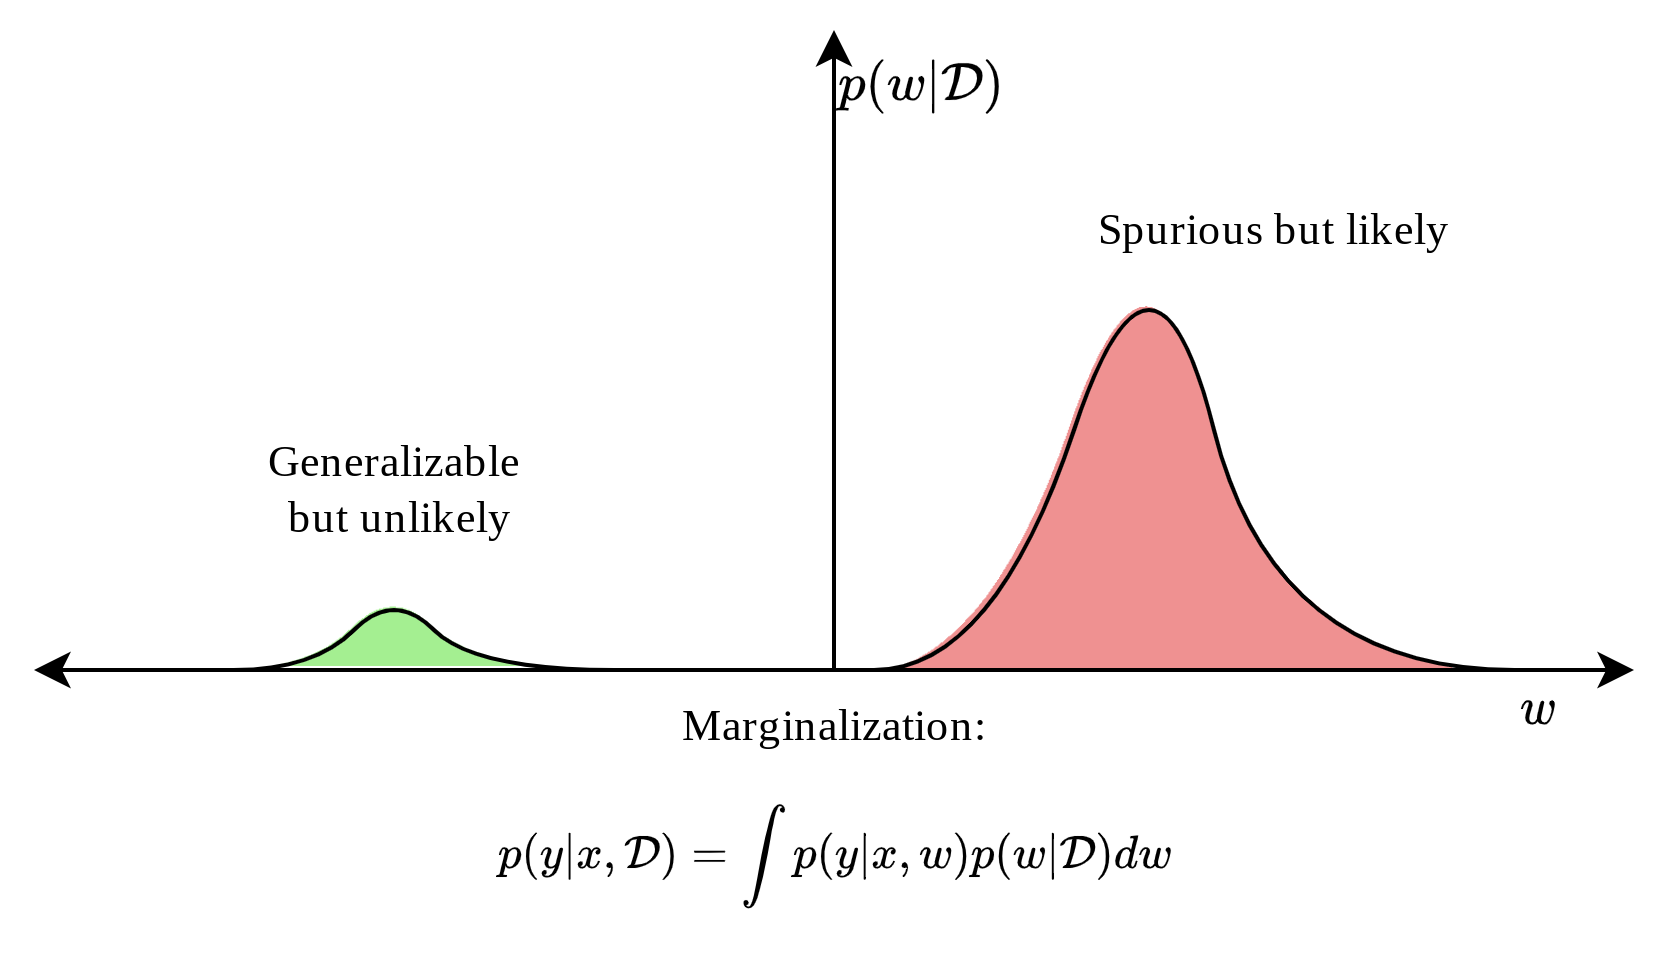
\includegraphics[width=\linewidth]{illustrations/bayesian.png}
    \caption[Bayesian Marginalization and Generalization]{Bayesian marginalization may not yield generalizable predictors. In the above case, the portion of the distribution that correspond to non-generalizable features (red) are more likely to be learned than generalizable features (green). Spurious features will as a consequence constitute the principal component of the marginalized probability, in turn resulting in minimal impact on generalization.}
    \label{fig:bayesian_generalization}
\end{figure}

\section{Ethical considerations}\label{ethics}
    Now that generalization failure and the prevalence thereof has been discussed in quite some detail, as well as limited success of the literature to address this, it is beneficial to pause to consider the ethical and social consequences inherent to the problem. 
    
    Naturally, the robustness and generalizability of medical systems is of exceptional importance~\cite{ethics_1}. The possible negative consequences for incorrectness or even simply unreliable performance are significant. Over-reliance on non-robust deep learning model may for instance result in increased miss rates, which of course may have fatal consequences should the polyp turn cancerous. Clinicians may grow accustomed to a high-performing model and then perhaps more readily fail to notice polyps left undetected by the model if for instance the distribution shifts such that this performance is hampered. In this case, the addition of the deep-learning based screening method would do more harm than good.
    
    As briefly mentioned in~\Cref{introduction}, sampling bias in the datasets upon which these models are trained may lead to inequality of treatment, for instance if certain demographics are not accounted for~\cite{social_consequence_1}. Though this of course can be mitigated to some extent by more careful curation of datasets, the central problem that results in this disparity is at its core the fact that the model is learning spurious features. A model intended to detect melanomas should not, for instance, rely solely on complexion-dependent characteristics to make predictions. Though curating datasets with a diverse representation of skin-tones would mitigate this problem to some extent, it is uncertain, and as the analysis in previous sections shows unlikely that all potential variability would be accounted for. Thus, ensuring that a given model learns causally robust and thus generalizable features is of particular importance also in these and similar contexts. 
    
    
\section{Summary}
This section has covered the basics of deep learning and segmentation, a number of documented cases of generalization failure, and summarized a number of analyses of generalization performed in the literature. The key takeaways can be summarized as follows: 

Generalization failure is prevalent across practically all deep learning pipelines. The mechanisms behind these failures are only loosely understood, and there has been limited success in the endeavors of developing generalizable predictors. Generalization failure can, however, in broad strokes be attributed to the inability of empirical risk minimization to consistently learn causal patterns, and that predictors trained with \gls{erm} instead favour whatever pattern that can be found in that is sufficiently predictive in a \gls{ind} context. Methods that address this in some way - for instance ensembles, data augmentation, etc - thus naturally appear to increase generalizability. 

The relative impact of these methods is, however, poorly understood, and the literature is to some extent fragmented with regards to the experimental methodology used when evaluating the generalizability of models. Moreover, there have been limited efforts made towards developing novel approaches explicitly aiming to increase generalization without relying on auxiliary \gls{ood} datasets in the training process. Hence, addressing this issues is the primary focus of this thesis.


